\section{Implementacja}
% Struktura translatora, opisać co się dzieje, dlaczego jest niezależne 
% itp., przepływ zapytania przez program
\begin{frame}
     \frametitle{Struktura}
\begin{center}
\includegraphics[height=70mm]{../diagramy/struktura.pdf}
\end{center}
\end{frame}


\begin{frame}
     \frametitle{Podział na moduły}
    
\begin{center}
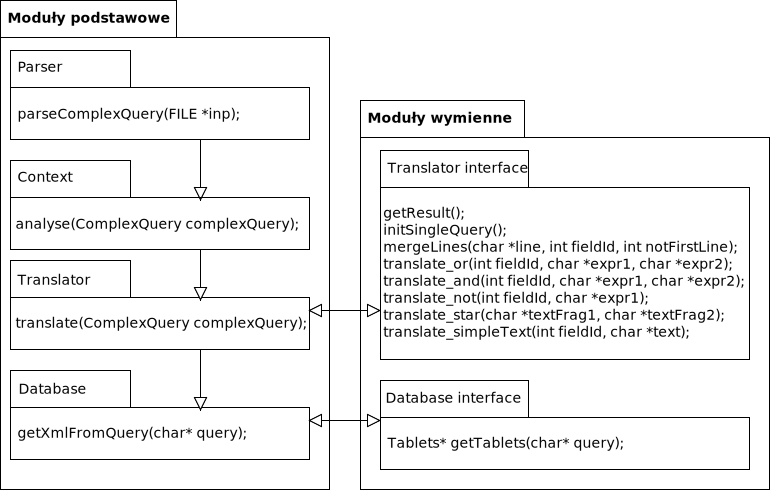
\includegraphics[width=100mm]{../diagramy/pakiety.pdf}
\end{center}
\end{frame}

\begin{frame}
\frametitle{Parser i analizator składniowy}
\begin{itemize}
\item \textbf{wejście} - zapytanie w języku TQL
\item \textbf{wyjście} - drzewo składni abstrakcyjnej
\item moduły niezależne od bazy danych i języka wyszukiwania
\item wspólne dla wszystkich implementacji TQL
\item napisane za pomocą narzędzia BNFC, następnie uporządkowane

\end{itemize}
\end{frame}

\begin{frame}
\frametitle{Translator}
\begin{itemize}
\item \textbf{wejście} - drzewo składni abstrakcyjnej
\item \textbf{wyjście} - zapytanie w odpowiednim języku
\item buduje zapytanie:
\begin{itemize}
 \item przechodzi strukturę drzewa
 \item wywołuje funkcje zależne od bazy danych (Translator\_interface.h)
 \item zwraca wynik (getResult())
\end{itemize}
\end{itemize}
\end{frame}


\begin{frame}
     \frametitle{Baza danych}
\begin{itemize}
\item \textbf{wejście} - zapytanie w języku docelowym
\item \textbf{wyjście} - XML zawierający informacje o znalezionych tabliczkach i ich treść
\item wykonuje zapytanie i tworzy wynik:
\begin{itemize}
\item przekazuje zapytanie do części zależnej od bazy danych (Database\_interface.h)
\item dostaje strukturę (Tablets)
\item otrzymaną strukturę przedstawia w postaci XML
\end{itemize}
\end{itemize}
\end{frame}

\begin{frame}
 \frametitle{Baza danych}
\begin{columns}[t]
\column{.5\textwidth}
\begin{block}{Struktura Tablet}
typedef struct\{ \\
~~~~char* id; \\
~~~~char* id\_cdli; \\
~~~~char* publication; \\
~~~~char* measurements; \\
~~~~char* year; \\
~~~~char* provenience; \\
~~~~char* period; \\
~~~~char* genre; \\
~~~~char* subgenre; \\
~~~~char* collection; \\
~~~~char* text; \\
~~~~Tags *tags; \\
\} Tablet; \\
\end{block}
\column{.5\textwidth}
\begin{block}{Struktura Tablets}
typedef struct\{ \\
~~~~int size; \\
~~~~Tablet *tabs; \\
\} Tablets;
\end{block}
\end{columns}

\end{frame}

\begin{frame}
 \frametitle{Dostosowanie do różnych baz danych}
\begin{itemize}
\item pliki zależne od bazy danych implementują interfejsy
\begin{itemize}
\item Translator\_interface.h
\item Database\_interface.h
\end{itemize}
\item istnieją dwie implementacje
\begin{itemize}
\item dla bazy relacyjnej PostgreSQL
\item dla bazy XML (Zorba)
\end{itemize}
\item równoczesna kompilacja poleceniem make
\end{itemize}
\end{frame}




